% 文件名:MainBody.tex
% 文件描述:四川大学2020研究生硕/博士 LaTeX 模版
% 作者:Kevin T. Lee [hello@lidengju.com]
% 修改日期:2020年6月1日
 
% 设置文档属性
% 参数说明
% professional: 专业学位
% academic: 学术学位
% master: 硕士
% doctor: 博士
% approval: 送审版本,将不生成声明
% secret: 保密论文,将显示密级
% color: 红色川大logo
% kfont=<⟨none|adobe|fandol|founder|mac|macnew|macold|ubuntu|windows|windowsnew|windowsold|...⟩>,
% 不填写则默认fandol
\documentclass[professional,master]{./Template/scuthesis2020}
\begin{document}
% 设置文档信息
\unitid{10610} % 单位代码
\STUnumber{xxxxxxxxxxxxxxx} % 学号或送审编号
\securityClassification{秘密} % 密级:公开/内部/秘密/机密/绝密。当不使用secret时,不显示
\securityYear{3} % 保密年限
\CoverTitle{论文标题可能很长} %封面标题
\CoverSubTitle{所以你可以把一部分放到副标题里} %可做封面副标题
\title{论文标题可能很长所以你可以把一部分放到副标题里} % 论文全称
\ENGtitle{Title of graduate thesis could be very very long but do not worry it will break the line automatically……} %论文全称英文
% \school{\zihao{5}{这里是特别长的单位名称甚至一行不能显示}} % 如果太长超出一行,可以根据显示效果修改字号,这里为5号字
\school{计算机学院} % 培养单位
\ENGschool{Computer Science} % 培养单位英文
\author{XXX} % 作者姓名
\ENGauthor{Kevin T. Lee} % 作者英文名
\supervisor{XXX\quad 教授} % 指导教师
\ENGsupervisor{Prof. XXX} % 指导教师英文
\degreeclass{工程硕士} % 学位类别
\ENGdegreeclass{Master of Engineering} % 学位类别英文
\major{计算机技术/具体领域} % 学科专业或领域名称
\ENGmajor{Computer Technology} % 学科专业或领域名称英文
\hasmajor{1} % 若有领域则为1,否则改为0
\defensedate{二〇二〇年二月} % 论文答辩时间
\grantdate{二〇二〇年二月} % 学位授予时间
\accomplishdate{二〇二〇年二月} % 论文完成时间
\statementdate{February, 2020} % 声明时间
\direction{XXX}
\ENGdirection{Direction Name}
\keywords{研究生学位论文;写作指南;参考模板}
\ENGkeywords{graduate thesis;writing guide;reference template}

% 自动制作封面
\maketitle
% 自动制作中英文声明
\makestatement
% 设置论文正文前的页码、页眉等
\frontmatter\pagenumbering{Roman}\pagestyle{fancy}
% 包含摘要
%!TEX root = ../MainBody.tex

% 中英文摘要
\begin{CHSabstract}
    学位论文是研究生科研工作成果的集中体现,是评判学位申请者学术水平、授予其学位的主要依据,是科研领域重要的文献资料。

博士学位论文表明作者在本门学科上掌握了坚实宽广的基础理论和系统深入的专门知识,在科学和专门技术上做出了创造性的成果,并具有独立从事创新科学研究工作或独立承担专门技术开发工作的能力。

硕士学位论文表明作者在本门学科上掌握了坚实的基础理论和系统的专业知识,对所研究课题有新的见解,并具有从事科学研究工作或独立承担专门技术工作的能力。

硕士专业学位论文表明作者在本专业领域掌握了重要的基础理论和系统的专门知识,对相关专业领域问题有新的见解,并具有解决实际问题的能力。

为提高研究生学位论文的撰写质量,促进学位论文在内容和格式上的规范化,根据《学位论文编写规则》(GB/T 7713.1-2006)和《信息与文献 参考文献著录规则》(GB/T 7714-¬2015)等国家有关标准,学院研究生办公室整理并撰写此文,作为指导性规范,供申请学位的研究生参考,以利于学位论文的撰写、收藏、存储、加工、检索和利用。

写作指南主要包括以下内容,分别为内容规范要求,格式规范要求,书写规范要求以及排版印制要求,同时提供了必要的相关附录材料。

本《写作指南与参考模板》将在使用过程中不断完善,如有问题和建议请及时向我们反馈,以便于改进。 谢谢!

\end{CHSabstract}

\begin{ENGabstract}
	\lipsum
\end{ENGabstract}


% 自动制作目录
\maketoc
% 自动制作图表目录
\makefigtablist
% 包含缩略词表
%!TEX root = ../MainBody.tex

% 常用缩略词表
\chapter{常用缩略词表}
\begin{appendix*}
\begin{tabular}{p{7em}p{25em}}
	Abbr. 1 & Abbreviation 1 \\
	Abbr. 2 & Abbreviation 2 \\
	Abbr. 3 & Abbreviation 3 \\
\end{tabular}
\end{appendix*}
% 包含符号表
%!TEX root = ../MainBody.tex

% 常用符号表
\chapter{常用符号表}
\begin{appendix*}
	\begin{tabular}{p{7em}p{20em}}
		$Symbol_{1}$ & 符号$1$ \\
		$Symbol_{2}$ & 符号$2$ \\
		$Symbol_{3}$ & 符号$3$ \\
	\end{tabular}
\end{appendix*}
% 设置论文正文部分的页码、页眉等
\mainmatter\pagenumbering{arabic}\pagestyle{fancy}
% 包含第一章、第二章等等
%!TEX root = ../MainBody.tex

% 第一章
\chapter{绪论}% 使用\cite{}命令引用数据库中文献
引言(或绪论)应包括选题的背景和意义,国内外相关研究成果与进展述评,本论文所要解决的科学与技术问题、所运用的主要理论和方法、基本思路和论文结构等。引言应独立成章,用足够的文字叙述,不与摘要雷同。要求实事求是,不夸大、缩小前人的工作和自己的工作。
\section{选题背景及意义}
要论述清楚为什么选择这个题目来研究,即阐述该研究对学科发展的贡献、对国计民生的理论与现实意义等。四川大学标志如\cref{fig:test1}所示。
%插入图片示例
\begin{figure}[!htb]
    \centering
    \begin{subfigure}[b]{0.6\textwidth}
    
\includegraphics[width=\textwidth]{./Template/Components/Images/SCU_TITLE}
    \bicaption{红色标志}{Red logo}
    \label{fig:sub_a}
    \end{subfigure}%
    \vspace{0.5cm}
    \begin{subfigure}[b]{0.6\textwidth}
        
\includegraphics[width=\textwidth]{./Template/Components/Images/SCU_TITLE_BW}
        \bicaption{黑色标志}{Black logo}
        \label{fig:sub_b}
    \end{subfigure}%
    \bicaption{四川大学标志}{Logo of Sichuan University}
    \label{fig:test1}
\end{figure}

% 另一种写法
\begin{figure}[!htb]
    % \ContinuedFloat % 用于子图连续编号,以实现子图跨页
    \centering
    \bisubcaptionbox
    {黑色标志\label{fig:test:A}}
    {Black logo}{
\includegraphics[width=4cm]{./Template/Components/Images/SCU_TITLE_BW}}%
    \qquad
    \bisubcaptionbox
    {红色标志\label{fig:test:B}}
    {Red logo}{ 
\includegraphics[width=4cm]{./Template/Components/Images/SCU_TITLE}}%
    \bicaption{四川大学标志}{Logo of Sichuan University}
    \label{fig:test2}
\end{figure}

\section{文献综述}
要对本研究主题范围内的文献进行详尽的综合述评,“述”的同时一定要有“评”,指出现有研究状态,仍存在哪些尚待解决的问题,讲出自己的研究有哪些探索性内容。曹敏\cite{曹敏GB,陈浩元2015gb}对修订后的GB/T 7714—2015《信息与文献参考文献著录规则》与上一版本GB/T 7714—2005《文后参考文献著录规则》的差异进行了分析,帮助读者尽快了解参考文献标准最新修订的内容。
\section{研究目的与实施方案}
讲述本论文运用的主要理论与研究方法、基本思路及论文的结构安排等。


%!TEX root = ../MainBody.tex

\chapter{结构内容}
\section{文字要求}
研究生学位论文(thesis or dissertation)应以汉语撰写(外国语言文学专业学位论文可以要求用其它文字撰写)。

来华留学生(全英文项目)可以用英文撰写学位论文,但须有详细中文摘要(不少于6000字),英文摘要300-800英文实词。
\section{结构组成}
学位论文一般由以下几部分内容构成,依次为:
\begin{itemize}
\item	中文封面 
\item	英文封面内页
\item	声明
\item	中英文摘要(关键词) 
\item	目录
\item	插图和附表清单(如有)
\item	符号、标志、缩略语等的注释表(如有)
\item	引言(绪论)
\item	正文
\item	参考文献
\item	附录(如有)
\item	攻读学位期间取得的研究成果
\item	致谢
\end{itemize}
\section{内容要求}
学位论文每部分应另页右页开始,各部分内容的要求如下:
\subsection{封面}
封面(cover)是学位论文的外表面,对论文起装潢和保护作用,并提供相关的信息。封面分为正式存档和匿名评审两种版式(参见前页),不同学位类别的论文封面分别使用学院指定的不同封面。

封面包含内容如下:

\textbf{单位代码:}10610

\textbf{学号(送审编号):}填写研究生学号。

\textbf{密级:}涉密论文必须在论文封面标注密级,同时注明保密年限。公开论文不标注密级,可删除。

\textbf{题目:}论文题目应以简明词语恰当、准确地反映出论文最重要的特定内容,通常由名词性短语构成,应尽量避免使用不常用缩略词、首字母缩写字、字符、代号和公式等。

如论文题目内容层次很多,难以简化时,可采用论文题目和论文副标题相结合的方法,主标题和副标题之间用破折号间隔。副标题起补充、阐明题目的作用。

示例1:斑马鱼和人的造血相关基因以及表观遗传学调控基因——进化、表达谱和功能研究

示例2:阿片镇痛的调控机制研究:Delta 型阿片肽受体转运的调控机理及功能

\textbf{培养单位:}指学位申请人学籍所在学院(所)名称,应规范填写全称。

\textbf{学科专业:}学科名称以国务院学位委员会颁布的《授予博士、硕士学位和培养研究生的学科、专业目录》为准,学术学位研究生的学位类别填写为:理(工、农)学博士或理(工、农)学硕士,学科专业填写为:一级学科-二级学科,如:生物学-动物学,生态学-动物生态学。专业学位研究生的学位类别填写为:林业硕士或工程硕士,领域名称填写:生物医学工程或生物工程,林业硕士未分设领域,填写:无。

\textbf{指导教师:}应填写经培养单位批准备案的的导师姓名,并加上专业技术职称(联合培养专项计划博士研究生填写双导师信息)。

\textbf{论文答辩时间/学位授予时间(论文完成时间):}填写举行毕业答辩和申请学位授予的时间,完成论文时间填写提交论文送审的时间。

\subsection{声明}
本部分放在学位论文原创性声明之后另起页,提交时须论文作者以及指导教师亲笔签名并填写日期。若申请学位时须对论文版本进行修改替换,须重新签名并填写日期。
\subsection{摘要(关键词)}
论文摘要包括中文摘要和英文摘要(Abstract)两部分。摘要是论文内容的简要陈述,是一篇具有独立性和完整性的短文,应概括地反映出本论文的主要内容,说明本论文的主要研究目的、内容、方法、成果和结论。要突出本论文的创造性成果或新见解,不宜使用公式、图表、表格或其他插图材料,不标注引用文献。中文摘要力求语言精炼准确,博士论文一般约为1000字(word统计),硕士论文一般约为600字(word统计)。英文摘要与中文摘要内容应完全一致。

摘要正文内容一般包括:从事这项研究工作的目的和意义;作者独立进行的研究工作的概括性叙述;研究获得的主要结论或提出的主要观点。硕士学位论文摘要应突出论文的新见解,博士学位论文摘要应突出论文的创新点。

关键词在摘要正文内容后另起一行标明,一般3~5个,之间用分号分开, 最后一个关键词后不打标点符号。关键词是为了文献索引和检索工作,从论文中选取出来,用以表示全文主题内容信息的单词或术语,应体现论文特色,具有语义性,在论文中有明确出处。应尽量采用《汉语主题词表》或各专业主题词表提供的规范词。
摘要页应单独编页。

\subsection{目录}
学位论文应有目录(目次) (table of contents)页,排在摘要之后,另起页。目录是论文各章节标题的顺序列表,附有相应的起始页码。目录应包括中英文摘要和论文正文中的全部内容的标题,以及参考文献、附录和致谢等。目录中的正文章节题名只编写到第三级标题,即×.×.×(如1.1.1)。一级标题顶格书写,二级标题缩进一个汉字符位置,三级标题缩进两个汉字符位置。

目录页应单独编页。

\subsection{图和附表清单(如有)}
论文中如有图表,应有图表目录,置于目录页之后,另页编排。图表目录应有序号、图题或表题和页码。
\subsection{符号、标志、缩略语等的注释表(如有)}
如果论文中使用了大量的物理量符号、标志、缩略词、专门计量单位、自定义名词和术语等,应编写成注释说明汇集表。若上述符号等使用数量不多,可以不设此部分,但必须在论文中首次出现时加以说明。
\subsection{正文}
正文一般包括引言(或绪论)、论文主体以及结论等部分,正文是学位论文的主体部分,应从另页右页开始,每一章应另起页。博士学位论文总字数不应少于6万字,正文部分不应少于5万字(word统计),硕士学位论文总字数不应少于3万字,正文部分不应少于2万字(word统计)。正文部分的篇幅(包括绪论、结论、图、表和公式),按照规范排版,硕士学位论文一般为40~60页,博士学位论文一般为80~120页。
\subsubsection{引言(或绪言)}
引言作为第一章,应包括:本研究的学术背景及理论与实际意义;国内外文献综述;本研究的来源以及研究目的、实施方案和主要研究内容与方法等。
\subsubsection{论文主体}
论文主体是正文的核心部分,占主要篇幅,它是将学习、研究和调查过程中筛选、观察和测试所获得的材料,经过加工整理和分析研究,进而形成论点。由于不同学科专业及具体选题的差异,此部分不作统一规定,可以按照章节体表述,也可以按照“前言-实验材料与方法-结果与讨论”的表述形式组织论文。但总体内容必须实事求是,客观真切,准确完备,合乎逻辑,层次分明,简练可读。
主体部分写作时,可参考以下结构(适用于几部分相对独立又有联系的研究内容):第1章 引言、第2章 ××××(第一部分研究内容)、第3章 ××××(第二部分研究内容)、第4章 ××××(第三部分研究内容)、第5章 结论与展望。每部分研究内容包括:材料与方法、结果以及讨论。

\subsubsection{结论与展望}
结论是对整个论文主要成果的总结,不是正文中各章小结的简单重复,应准确、完整、明确、精炼。应明确指出本研究的创新点,对论文的学术价值和应用价值等加以预测和评价,说明本项研究的局限性或研究中尚难解决的问题,并提出今后进一步在本研究方向进行研究工作的设想或建议。

结论部分应严格区分本人研究成果与他人科研成果的界限。

\subsection{参考文献}
本着严谨求实的科学态度撰写论文,凡学位论文中有引用或参考、借用他人成果之处,均应按不同学科论文的引用规范,列于文末(通篇正文之后),严禁抄袭剽窃。

参考文献列示的内容务必实事求是。论文中引用过的文献必须著录,未引用的文献不得虚列。遵循学术道德规范,杜绝抄袭、剽窃等学术不端行为。

参考文献应有权威性,并注意所引文献的时效性。

参考文献的数量:硕士学位论文,不少于60篇,其中,国外文献不少于30篇,应以近5年的文献为主;博士学位论文,不少于100篇,其中,国外文献不少于50篇,应以近5年的文献为主。

\subsection{附录(如有)}
主要列入正文内过分冗长的公式推导,供查读方便所需的辅助性数学工具或表格,重复性数据图表,论文使用的缩写,程序全文及说明等。
\subsection{致谢}
致谢中主要感谢导师和对论文工作有直接贡献和帮助的人和单位。对象一般为:指导或协助指导完成论文的导师;资助基金、合同单位、其他提供资助或支持的企业、组织或个人;协助完成研究工作和提供便利条件的组织或个人;在研究工作中提出建议和提供帮助的人;给予转载和引用权的资料、图片和文献等,研究思路和设想的所有者。
致谢用语应谦虚诚恳,实事求是。字数不超过1000字(word统计)。

\subsection{攻读学位期间取得的研究成果}
按研究成果发表的时间顺序,列出作者本人在攻读学位期间已发表或已正式录用待发表的成果清单(著录格式同参考文献)。成果形式可为学术论文、申请的专利、获得的奖项及完成的项目等。
%!TEX root = ../MainBody.tex

\chapter{书写规范}
\section{文字、标点符号和数字}
汉字的使用应严格执行国家的有关规定,除特殊需要外,不得使用已废除的繁体字、异体字等不规范汉字。标点符号的用法应该以GB/T 15834—1995《标点符号用法》为准。数字用法应该以GB/T 15835—1995《出版物上数字用法的规定》为准。
\section{章节及各章标题}
论文正文须由另页右页开始。分章节撰写时每章也为另页右页开始,论文排版时注 意让每一章节的最后一页尽量不出现空白页面。各章标题中尽量不采用英文缩写词,尽 量不使用标点符号。
\section{序号}
\subsection{标题序号}
论文标题分层设序。层次以少为宜,根据实际需要选择。各层次标题一律用阿拉伯数字连续编号;不同层次的数字之间用小圆点“.”相隔,末位数字后面不加点号,如“1.1”,“1.1.1”等;章的标题居中排版,各层次的序号均左起顶格排,后空一个字距接排标题。例如:
\begin{figure}[!hbp]
    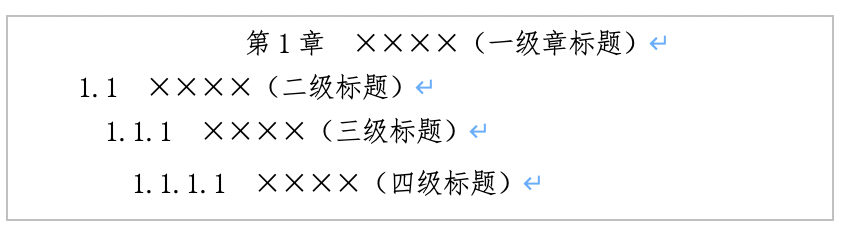
\includegraphics[width=13cm]{./Figures/levels}
    \centering
    \bicaption{图标题}{Title}
    \label{fig:levels}
\end{figure}
\subsection{图表等编号}
论文中的图、表、附注、公式、算式等,一律用阿拉伯数字分章依序连续编码。其 标注形式应便于互相区别,如:图 l.1(第 1 章第一个图)、图 2.2(第 2 章第二个图);3.2(第 3 章第二个表)等。
\subsection{页码}
页码从引言(或绪论)开始按阿拉伯数字(1,2,3……)连续编排,页码位于页 面下方居中、右页右下角;此前的部分(中、英文摘要、目录等)用大写罗马数字(I, II, III…)单独编排, 页码位于页面下方居中。
\subsection{页眉}
\section{名词和术语}
\section{量和单位}
\section{图和表}
\subsection{图}
插图须紧跟文述。在正文中,一般应先见图号及图的内容后再见图,一般情况下不能提前见图,特殊情况须延后的插图不应跨节;提供照片应大小适宜,主题明确,层次清楚,金相照片一定要有比例尺;图应具有“自明性”,即只看图、图题和图例,不阅读正文,就可理解图意。引用的图必须注明来源。

图的大小一般为宽6.67 cm×高5.00cm。特殊情况下,也可宽9.00 cm×高6.75cm,或宽13.5 cm×高9.00cm。同类图片的大小应尽量一致,编排美观、整齐。如\cref{fig:demo}
\begin{figure}[H]
    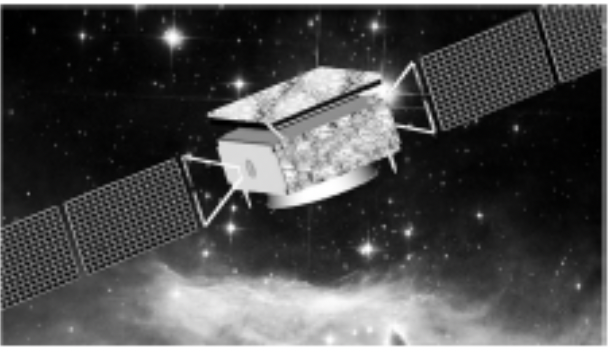
\includegraphics[width=9cm]{./Figures/demo}
    \centering
    \bicaption{图标题}{Title}
    \label{fig:demo}
\end{figure}
一幅图如有若干幅分图,均应编分图号,用(a),(b),(c),...... 按顺序编排,且各分图的分题注直接列在各自分图的正下方,总题注列在所有分图的下方正中。
\subsection{表}
表的编排一般是内容和测试项目由左至右横读,数据依序竖排,应有自明性,引用的表必须注明来源。具体要求如下:

每一表应有简短确切的题名,连同表序号置于表上居中。必要时,应将表中的符号、标记、代码及需说明的事项,以最简练的文字横排于表下作为表注。论文表的题名需用中文及英文两种文字表达,表注可用中英文两种文字表达或只用中文表达。

表内同一栏数字必须上下对齐。表内不应用“同上”、“同左”等类似词及“″”符号,一律填入具体数字或文字,表内“空白”代表未测或无此项,“—”或“…”(因“—”可能与代表阴性反应相混)代表未发现,“0”该表实测结果为零。

表格尽量用“三线表”,避免出现竖线,避免使用过大的表格,确有必要时可采用卧排表,正确方位应为“顶左底右”,即表顶朝左,表底朝右。表格太大需要转页时,需要在续表表头上方注明“续表”,表头也应重复排出。
表中用字为五号字体。如排列过密,用五号字有困难时,可小于五号字,但不小于七号。表格必须通栏,即表格宽度与正文版面平齐。
示例:
\begin{table}[htp]
    \bicaption{表标题}{Title}
	\centering
    % 调整表格,修改数字即可
    % \resizebox{\textwidth}{12mm}{ % 表格过宽
	\setlength{\tabcolsep}{1cm}{ %表格过窄
	\zihao{5}
	\begin{tabular}{cccc}
    \toprule
    文献类型  & 标志代码 & 文献类型 & 标志代码 \\
    \midrule
    普通图书  & M    & 会议录  & C    \\
    汇编    & G    & 报纸   & N    \\ 
    期刊    & J    & 学位论文 & D    \\
    报告    & R    & 标准   & S    \\
    专利    & P    & 数据库  & DB   \\
    计算机程序 & CP   & 电子公告 & EB   \\
    \bottomrule
    \end{tabular}}
    \label{tab:demo}    
\end{table}
\section{表达式(公式)}
论文中的公式应另起一行,居中编排,较长的公式尽可能在等号后换行,或者在“+”、“-”等符号后换行。公式中分数线的横线,长短要分清,主要的横线应与等号取平。公式后应注明编号,公式号应置于小括号中,如公式(2-3)。写在右边行末,中间不加虚线;公式下面的“式中:”两字左起顶格编排,后接符号及其解释;解释顺序为先左后右,先上后下;解释与解释之间用“;”隔开。

公式中各物理量及量纲均按国际标准(SI)及国家规定的法定符号和法定计量单位标注,禁止使用已废弃的符号和计量单位。
示例:
\begin{equation}
\label{eq:demo}
q=k_dH^x
\end{equation}
式中:q\cdash 灌水器流量/L·h-1;kd\cdash 流量系数;H\cdash 工作压力/m;x\cdash 流态指数。 

(此处,“式中:”改为顶格输出)

\section{算法(伪代码)}
本节介绍了一个伪代码示例,如\cref{alg:alg1}所示。
\begin{algorithm}
	\caption{Calculate $y = x^n$} 
	\label{alg:alg1}
	\begin{algorithmic}[1]
		% 输入
		\REQUIRE $n \geq 0 \vee x \neq 0$ 
		% 输出
		\ENSURE $y = x^n$ 
		
		% 初始化
		\STATE $y \leftarrow 1$ 
		
		% 逻辑
		\IF{$n < 0$} 
			\STATE $X \leftarrow 1 / x$ 
			\STATE $N \leftarrow -n$ 
		\ELSE 
			\STATE $X \leftarrow x$ 
			\STATE $N \leftarrow n$
		\ENDIF
		
		\WHILE{$N \neq 0$} 
			\IF{$N$ is even} 
				\STATE $X \leftarrow X \times X$ 
				\STATE $N \leftarrow N / 2$ 
			\ELSIF{$N$ is odd}
				\STATE $y \leftarrow y \times X$ 
				\STATE $N \leftarrow N - 1$ 
			\ENDIF 
		\ENDWHILE
	\end{algorithmic}
\end{algorithm}

\section{参考文献}
参照GB/T 7714—2015《信息与文献 参考文献著录规则》执行。
\section{附录}
附录编号依次为附录A,附录B。附录标题各占一行,按一级标题编排。每一个附录一般应另起一页编排,如果有多个较短的附录,也可接排。附录中的图、表、公式另行编排序号,与正文分开,编号前加“附录A-”字样。
附录作为主体部分的补充(不是必需的)。下列内容可作为附录编于论文后。

——为了整篇论文材料的完整,但编于正文又有损于编排的条理性和逻辑性,这一材料包括比正文更为详尽的信息、研究方法和技术更深入的叙述,以及对了解正文内容有用的补充信息等。

——由于篇幅过大或取材于复制品而不便于编入正文的材料。

——不便于编入正文的罕见珍贵资料。

——对一般读者并非必要阅读,但对本专业同行有参考价值的资料。

——正文中未被引用但被阅读或具有补充信息的文献。

——某些重要的原始数据、数学推导、结构图、统计表、计算机打印输出件等。

%!TEX root = ../MainBody.tex

\chapter{排版打印}
\section{纸张规格和页面设置}
\section{中文封面排版说明}
\section{中、英文摘要排版要求}
\section{目录排版要求}
\section{正文排版要求}
\section{其他部分排版要求}
\section{评阅送审论文版式要求}
采用评阅送审论文封面格式,删除英文封面内页、声明页、致谢,攻读学位期间取得的研究成果参照写作指南的说明进行备注,其它格式参照《研究生学位论文规范写作指南》的要求。 
\section{论文印刷及装订要求}
论文自中文摘要起双面印刷,之前部分单面印刷,之后各部分须由另页右页开始(排版时注意微调,左页不要出现空白页)。论文须用热胶装订。博士(学术学位)论文封面颜色为红色,硕士(学术学位)论文封面颜色为蓝色,硕士(专业学位)论文封面颜色为绿色。
%!TEX root = ../MainBody.tex

\chapter{结论与展望}
结论是对论文主要研究结果、论点的提炼与概括,应准确、简明、完整、有条理,使人看后就能全面了解论文的意义、目的和工作内容。主要阐述自己的创造性工作及所取得的研究成果在本学术领域中的地位、作用和意义。

结论要严格区分自己取得的成果与导师及他人的科研工作成果。在评价自己的研究工作成果时,要实事求是,除非有足够的证据表明自己的研究是“首次”的、“领先”的、“填补空白”的,否则应避免使用这些或类似词语。 

展望或建议,是在总结研究工作和现有结论的基础上,对该领域今后的发展方向及重要研究内容进行预测,同时对所获研究结果的应用前景和社会影响加以评价,从而对今后的研究有所启发。

% 设置论文正文后的式样
\backmatter
% 按国标自动制作参考文献
% 参考文献数据文件为本目录下的ReferenceBase.bib
\begin{reference}
	\bibliography{ReferenceBase}
\end{reference}
% 包含在读期间科研成果
%!TEX root = ../MainBody.tex

% 作者在读期间科研成果简介
\chapter{攻读学位期间取得的研究成果}
已发表或已录用的学术论文、已出版的专著/译著、已获授权的专利按参考文献格式 列出。未确定正式录用待发表的成果,不能写入此部分内容,成果若为录用待发表状态, 请备注。科研获奖,列出格式为:获奖人(排名情况).项目名称.奖项名称及等级, 发奖机构,获奖时间。与学位论文相关的其它成果参照参考文献格式列出。

全部研究成果连续编号编排。

\textcolor{red}{
    说明:评语送审版本,须保留此页,已取得的研究成果,按照以下内容进行备注:
\\
    “攻读学位期间所取得的研究成果,以第一作者身份(或其他身份)已在《******》 SCI 期刊/核心期刊上正式发表(或被《******》SCI 期刊/核心期刊正式录用待发表), 按照双盲评阅的要求,成果的详细信息未在此匿名评审论文中列出。”
}

% 包含致谢
\makethanks
\end{document}
